\usepackage{lipsum}
\usepackage{mathrsfs}
\usepackage{amsmath}
\usepackage{amssymb}
\usepackage{soul}

%%%%%%%%%% MULTI COLUMNS related %%%%%%%%%
\usepackage{multicol}
\usepackage{paracol}
%%%%%%%%%%%%%%%%%%%%%%%%%%%%%%%%%%%%%%%%%%

%%%%%%%%% TIKZ related %%%%%%%%%%%%
%\usetikzlibrary{shapes, snakes, arrows, arrows.meta, positioning, backgrounds}
%\usepackage{geometry}
%%%%%%%%%%%%%%%%%%%%%%%%%%%%%%%%%%%%%%%%%%%%

\begin{document}

% =======================================================================================
%\cleardoublepage % Forces the first chapter to start on an odd page so it's on the right

% =======================================================================================
%                                   PREAMBLE
% =======================================================================================
\coverpage{\TITLE}{\SUBTITLE}{\AUTHOR}{\DATE}{\SUBJECT}
%----------------------------------------------------------------------------------------
\newpage
\begin{center}
    \Large$\mathfrak{PREFACE}$
\end{center}

This practical guide on \textit{Spiking Neural Networks} (SNNs) is meant for Neuromorphic Computing enthusiasts and budding researches (with zero to basic-level proficiency)
in SNNs. In this first edition of the book, we have covered only the most well-established and widely accepted theories in SNNs. Therefore, this book is written to be introductory in nature, such that - after reading it, you can expect yourself to be at ease while reading most of the spiking networks literature. Note that as of this writing, research in SNNs is a rapidly growing domain and hasn't quite matured as that of the Deep Neural Networks (DNNs). Therefore, you might find that some (recent) popular theories in SNN literature have not been covered in this book; we intend to incorporate them in the later editions.

You ask \textit{why write this book?}

Research in SNNs is in relatively nascent stage; and although we have a growing number of literature on it, they aren't organized well. We have also noted the dearth of university level courses on SNNs -- they aren't as ubiquitous as courses on Deep Learning. Consequently, novice researchers generally struggle to \textit{Getting started with SNNs}. Herein, we present an organized collection of the basics of building and training various kind of spiking networks, introduction to popular neuromorphic chips, and related \texttt{PyScript} code examples that can be natively run on your own browsers! Additionally, we also point to a few popular research papers when we feel its necessary to dive into the theoretical details.

\textit{Prerequisites to reading this book --}

We recommend the readers to have familiarity with undergraduate level of \textit{Deep Learning} and \textit{Signals \& Systems}, basic \textit{Python} programming, and basic-to-intermediate level of experience with \textit{PyTorch} - for getting the most of this book; although, we do provide Appendices when necessary.
\\
\linebreak
\linebreak
\linebreak
\textit{We hope this book embarks you on the rewarding journey of researching in spiking networks!}

-- Authors
\tableofcontents

% =======================================================================================
%                                   PART I
% =======================================================================================
\part{Computational Neuroscience}
%----------------------------------------------------------------------------------------
\newpage
\chapter{Spiking Neurons} \label{ch:spk-neurons}
In this chapter, we will study the most fundamental unit of building SNNs -- the \textbf{Spiking Neurons}. When it comes to the SNNs, you may think of \textsl{Spiking Neurons} as \textit{analogous} to the \textsl{Artificial Neurons} in the DNNs. This chapter starts with a section on the \textsl{Biological Neurons} that lay down the neuroscience principles underlying the spiking neurons. Later, a section on the \textit{functional comparison} between spiking neurons and artificial neurons is also presented, where we highlight the inherent temporality and sparsity of spiking neurons.

\subsection{Should we write a section on why Spiking Neurons}
Sparse method of encoding and working with temporal information. H/W neurons don't need to be active all the time.

\section{Dales Principle}
and How SNNs violate that?

\section{Biological Neurons} \label{sec:bio-neuron}
\subsection{Action Potentials}
Perhaps look here: 

\url{https://pure.rug.nl/ws/portalfiles/portal/1106997626/Complete_thesis.pdf}

Introduce the notations for membrane potential, V[t], input current I[t], etc. here and then explain them in the Spiking Neurons section.


\newpage
\section{Spiking Neurons}
\textbf{Spiking Neurons} are electro-mathematical abstraction of biological neurons. They are generally \textit{not} very detailed representations of biological neurons, rather simple enough to reproduce their intended spiking behaviour. Note that a majority of the spiking neurons you will come across will fall into the category of \textsl{point} spiking neuron models; few rare ones will fall into the category of \textsl{spatial} spiking neuron models. The \ul{major characteristics} of biological neurons -- that are of common interest to mimic (via spiking neurons) are:
\begin{itemize}
    \item \ul{Accounting incoming action-potentials}: % https://www.perplexity.ai/search/in-the-biological-neurons-what-47xWVzh_Td.1IE1ppBqXYQ
    Spiking neurons emulate this behavior by \textit{integrating} the incoming action-potentials into their membrane potential/voltage -- either in a \textit{decaying} or \textit{non-decaying} fashion (more details later). Assuming the incoming action-potentials positively contribute, the spiking neuron's potential/voltage increases with time and eventually reaches/crosses a certain set voltage threshold.
    \vspace{5pt}
    
    \item \ul{Generating an output action-potential}: %Biological neurons generate action potential by aggregating inputs from its \textit{dendrites} on the \textit{soma}. 
    Spiking neurons emulate the generation of action-potential by %aggregating the inputs from its pre-synaptic neurons and 
    producing a \textit{binary}/\textit{graded} \textsl{spike}, where a \textit{binary} \textsl{spike} implies a binary value $\in \{0, 1\}$ and a \textit{graded} \textsl{spike} implies an integer value $\in \mathbb{Z}^+ > 1$. Note that the values of spikes are also sometimes referred as their \textit{amplitude}.
    \begin{remark}
        Some SNN implementations may use negative spikes! Also, it is commonly agreed that biological neurons' action potentials do \textit{not} have the notion of amplitude.
    \end{remark}
    \vspace{5pt}
    
    \item \ul{Resetting the membrane potential}: Spiking neurons emulate the resetting of membrane potential/voltage via two common methods: \textsl{hard-reset} and \textsl{soft-reset}, %where the membrane potential/voltage of a neuron that spiked (i.e., generated a spike) is immediately \textit{reset}. 
    where \textsl{hard-reset} implies setting the neuron's voltage to $0$, whereas \textsl{soft-reset} implies setting the neuron's voltage to a value that is equal to the neuron's current voltage \textit{subtracted} by its assumed voltage threshold. The difference between these two will be clear in the later sections.
    \vspace{5pt}
    
    \item \ul{Entering into refractory state}: Spiking neurons emulate this behavior by generally keeping their membrane potential/voltage at $0$ (in case of soft-reset) or at a subtracted value (in case of hard-reset) for a certain number of time-steps. This characteristic is typically ignored while building SNNs and is subject to varied implementations.
    \vspace{5pt}
    
    \item \ul{Propagating the action-potential along axon}: Spiking neurons generally do \textit{not} emulate this behaviour, except for the \textsl{spatial} spiking neuron models. This characteristic/property is typically embedded into the SNNs itself via the concept of \textit{delays}. In other words, when an action-potential propagates along the neuron's axon, it reaches the axon-terminal typically after some delays; this behaviour is accommodated in SNNs via introducing delays in spike propagation between the pre-synaptic and post-synaptic layers.
\end{itemize}

\subsection{Point Spiking Neuron Models}
\textbf{Point spiking neurons} are minimalistic neuron models that use simplified electro-mathematical equations to mimic the spike generation, voltage reset, and refractory state behaviour of biological neurons; they conveniently ignore to model the ionic channels, axial conductance, axonal propagation of spike/action-potential, etc., basically anything that relates to the spatial form of a biological neuron. Common examples of point spiking neurons are \textsl{Integrate \& Fire}, \textsl{Leaky Integrate \& Fire}, and \textsl{Resonate \& Fire} neuron models. 
\subsubsection{Integrate \& Fire neuron model}
\textbf{Integrate \& Fire} (IF) neuron model is the simplest of all the spiking neuron models -- by virtue of which, it's dynamic behaviour is also quite limited. An IF neuron, as the name goes, (at the very least) \textit{integrates} the incoming/input spikes into its \textit{non-decaying} membrane potential/voltage, followed by generating an output spike when its voltage reaches/crosses the set voltage threshold; whether or not it undergoes through a refractory state, is dependent on the subjective implementation. Following is the \textit{continuous-time} equation of an IF neuron: 
\begin{align}
C\frac{dV(t)}{dt} &= I(t) \\
\end{align}
Note the inherent temporality in $t$.

To implement an IF neuron on digital systems, i.e., your computer, it is necessary to discretize its continuous-time equations. Following are the \textit{discrete-time} equations (i.e., Eqs \eqref{eq:discrete-if-cur-update}, \eqref{eq:discrete-if-vol-update}, \eqref{eq:discrete-if-spk-out}, \& \eqref{eq:discrete-if-v-reset}) that describe an IF neuron: 

\begin{highlight}
\vspace{-10pt}
\begin{align}
I[t] &= (1 - \tau_\text{cur})\times I[t-1] + w\times S_\text{inp}[t] \label{eq:discrete-if-cur-update} \\
V[t] &= V[t-1] + I[t] \label{eq:discrete-if-vol-update}\\
S_\text{out}[t] &= \Theta(V[t] - V_\text{thr}) \label{eq:discrete-if-spk-out} \\
V[t] &\leftarrow V_\text{rest} \text{\qquad\qquad$\cdots$ if $V[t]>V_\text{thr}$} \label{eq:discrete-if-v-reset}
\end{align}
\end{highlight}

Before we begin explaining them, consider a \textsl{Spike Generator} that generates binary spikes $S_\text{inp}[t]$ (i.e., $S_\text{inp}[t]$ at time-step $t$ can either be $0$ or $1$) and feeds them to the IF neuron (see Fig \ref{fig:spk-neuron:if}). Note that spike generators are mere \textit{programming constructs} (that follow a desired implementation) to generate spikes and stimulate the connected neuron(s).

\begin{figure}[h]
    \centering
    \begin{tikzpicture}[
    spk-gen/.style={draw, star, very thick, fill=red!50, minimum width=0.5cm, scale=1.25},
    neuron/.style={draw, circle, very thick, fill=orange!40, scale=2, thick, inner sep=1pt}
    ]
    % Draw nodes.
    \node[spk-gen, label=below:\shortstack{\texttt{Spike}\\\text{Generator}}] (SpkGen) at (0,0) {};
    \node[neuron, label=below:\texttt{IF Neuron}] (IF-neuron) at (4,0) {\tiny $\curlywedge$};

    % Draw connections.
    \path[->] (SpkGen) edge [very thick] node[below] {$w$} (IF-neuron);
    
    \end{tikzpicture}
\caption{A \texttt{Spike Generator} stimulating an \texttt{IF Neuron}. $w$ is the weight of connection.}
\label{fig:spk-neuron:if}
\end{figure}

% \setcolumnwidth{0.7\textwidth, 0.3\textwidth}
% \begin{paracol}{2}
% First column:
% \switchcolumn
% Second column:
% \end{paracol}

In the Eq \eqref{eq:discrete-if-cur-update}, $I[t]$ and $I[t-1]$ are the IF neuron's \textit{current} at time-step $t$ and $t-1$, $\tau_\text{cur}$ is the \textit{current decay} constant (s.t., $0\leq\tau_\text{cur}\leq1$). As can be seen in the \textit{current update} Eq \eqref{eq:discrete-if-cur-update}, the current at time-step $t$ i.e., $I[t]$ is a sum of the \textit{decayed} value of current at the previous time-step $t-1$ i.e., $I[t-1]$ (decayed by the factor $(1 - \tau_\text{cur})$) \ul{and} the $w$ weighted spike input $S_\text{inp}[t]$.

In the Eq \eqref{eq:discrete-if-vol-update}, 


where, $S_\text{inp}[t]$ are the \textit{input} spikes from the preceding/pre-synaptic neuron to the IF neuron, $I[t]$ and $V[t]$ are the IF neuron's \textit{current} and \textit{voltage} respectively -- all at the \textit{discrete} time-step $t$. Note that $I[t-1]$ and $V[t-1]$ are the IF neuron's current and voltage at the previous time-step `$t-1$' -- accounting these values realizes the stateful-ness of the IF neuron. Also note that the current $I[t]$ intakes a , where , whereas, there is no such decay term for $V[t]$'s update.

\subsubsection{Leaky Integrate \& Fire Neuron Model}
\begin{remark}
    Most of the literature on SNNs use point neuron models because they are simple and easy to implement in both software and hardware.
\end{remark}

\begin{highlight}
Some highlight
\end{highlight}
\subsection{Spatial Spiking Neuron Models}
\subsubsection{Hodgkin Huxley Neuron Model}

\begin{remark}
Here is some remark \ref{sec:proin}.
\end{remark}

\newpage % Otherwise the paragraph overlaps with the text in the vertical ribbon.
\paragraph{Spiking Neurons Summary}
Example of a website \href{https://example.com/}{example.com}.
%----------------------------------------------------------------------------------------
\newpage
\chapter{Encoding \& Decoding}\label{ch:enco-deco}
\section{Whys, Whats, and Hows of Encoding \& Decoding} \label{sec:proin}

\subsection{Encoding}

{{#plot}}
---
title: Hi
---
def simulate(x, y):
    return x**2
{{/plot}}

\begin{figure}[hb]
\centering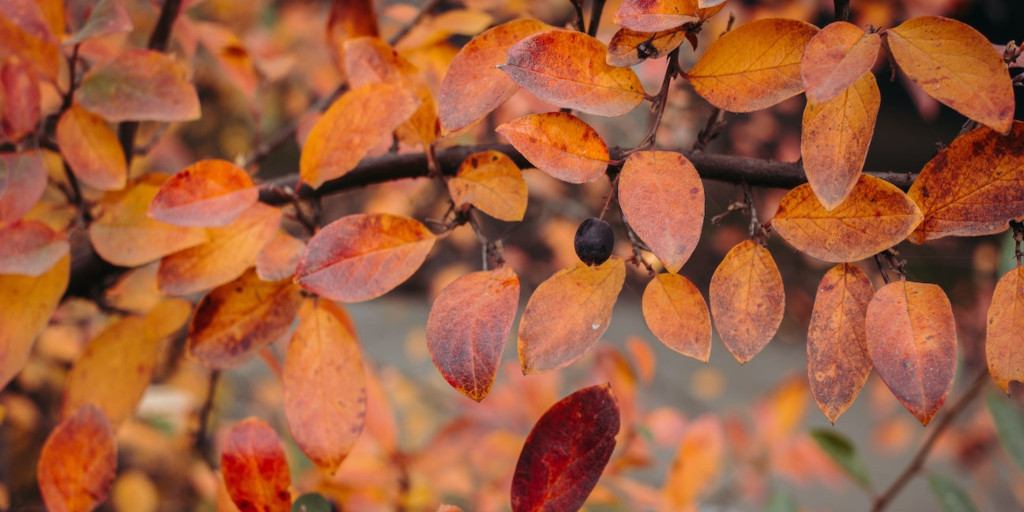
\includegraphics[scale=1]{images/orange2.jpg}
\caption{Caption of a Figure} 
\label{fig:integer}
\end{figure}

\subsection{Decoding}
See Fig \ref{fig:integer} above.

%----------------------------------------------------------------------------------------
\newpage
\chapter{Spiking Networks}\label{ch:spk-networks}
\input{sections/part1/spiking_networks}

%----------------------------------------------------------------------------------------
\newpage
\chapter{Modeling Theories}\label{ch:mdlng-theo}
\section{Neural Engineering Framework \label{sec:nef}}


\subsection{Representation Principle}
\subsection{Transformation Principle}
\subsection{Dynamics Principle}

\section{PRIMs}

% =======================================================================================
%                                   PART II
% =======================================================================================
\part{Spiking Neural Networks}
%----------------------------------------------------------------------------------------
\newpage
\chapter{Types of Spiking Neural Networks} \label{ch:snn-types}
\section{Feed-forward SNNs} \label{sec:sed-ultrices}

\subsection{Sub Section 1}


\begin{enumerate}
\item{List item -1}
\item{List item -2}
\item{List item -3}
\item{List item -4}
\end{enumerate}

\subsection{Subsection 2}

\begin{outline}
\lipsum[3]
\end{outline}

\subsection{Code Section}

\begin{lstlisting}[language=Solidity]
contract KingOfTheHill is Ownable {
    address public owner; // different from the owner in Ownable

    function () public payable {
        if(msg.value > jackpot) owner = msg.sender; // local owner
        jackpot += msg.value;
    }
    function takeAll () public onlyOwner { // contract creator
        msg.sender.transfer(this.balance);
        jackpot = 0;
    }
}
\end{lstlisting}

%----------------------------------------------------------------------------------------
\newpage
\section{Convolutional SNNs} \label{sec:conv-snns}

Refer Flowchart \ref{fig:flow-chart}.

\begin{figure}[ht]
\hspace*{-1.6cm}
\begin{tikzpicture}

\node (logs) [io] {Logs};
\node (storage) [io, right=2cm of logs] {Storage};
\node (log-topics) [io, below=1cm of logs] {Log: topics, data};

\node (parse-data) [block, below=1cm of log-topics] {Parse event arguments};
\node (arguments) [io, below=2.7cm of parse-data] {Event arguments};

\node (parse-selector) [block, left=2cm of parse-data] {Parse event selector};
\node (reverse-selector) [block, below=1cm of parse-selector] {Reverse selector};
\node (signature) [io, below=1cm of reverse-selector] {Event signature};

\node (identify-standard) [block, below=1cm of signature] {Identify standard and event};
\node (fetch-constraints) [block, below=1cm of identify-standard] {Fetch matching constraints};
\node (check-constraints) [decision, below=4.3cm of arguments] {Constraints?};

\node (references) [io, left=1.6cm of identify-standard] {References};
\node (rules) [io, left=2cm of fetch-constraints] {Rules};

\node (negative) [io, below=2cm of check-constraints] {False};
\node (positive) [io, right=2cm of negative] {True};

\node (c1) [container, fit=(parse-selector) (reverse-selector) (parse-data), draw=gray] {};

\node (c2) [container, fit=(identify-standard) (fetch-constraints), draw=gray] {};

\node (c3) [container, fit=(positive) (negative)] {};

\node (c4) [container, fit=(references) (rules)] {};

\node (c0) [container, fit=(log-topics) (c1) (c2) (check-constraints), inner ysep=6mm, yshift=-2mm] {};
\node (t0) [cstm-label, above=2mm of c0, xshift=-4cm] {Event poisoning?};

\draw [cstm-arrow] (logs) -- (log-topics);
\draw [cstm-arrow] (log-topics) -| (parse-selector);
\draw [cstm-arrow] (log-topics) -- (parse-data);
\draw [cstm-arrow] (parse-selector) -- (reverse-selector);
\draw [cstm-arrow] (reverse-selector) -- (signature);
\draw [cstm-arrow] (signature) -- (identify-standard);
\draw [cstm-arrow] (parse-data) -- (arguments);
% \draw [arrow] (arguments) |- (identify-standard);
\draw [cstm-arrow] (arguments) -- (check-constraints);
\draw [cstm-arrow] (identify-standard) -- (fetch-constraints);
\draw [cstm-arrow] (fetch-constraints) |- (check-constraints);
\draw [cstm-arrow] (references) -- (identify-standard);
\draw [cstm-arrow] (rules) -- (fetch-constraints);
\draw [cstm-arrow] (storage) -- +(0,-9cm) -| (check-constraints);
\draw [cstm-arrow] (check-constraints) -| node[cstm-label, near start, above] {no} (positive);
\draw [cstm-arrow] (check-constraints) -- node[cstm-label, near start, right] {yes} (negative);

\draw [cstm-arrow] (logs) edge [loop above] node[cstm-label, above] {Iterate} ();

\end{tikzpicture}
\caption{Some Flowchart} 
\label{fig:flow-chart}
\end{figure}


\section{Recurrent SNNs}
%----------------------------------------------------------------------------------------
\newpage
\chapter{Training Spiking Neural Networks} \label{ch:snn-trng}
\section{Neuro-inspired learning methods}
\subsection{Hebbs Law}
\subsection{Dale's Principle}
\subsection{STDP}
\subsection{R-STDP}

\section{Deep Learning -inspired methods}
\subsection{ANN-to-SNN Conversion}
\subsection{Surrogate Gradient Descent}

% =======================================================================================
%                                   PART III
% =======================================================================================
\part{Neuromorphic Hardware}
%----------------------------------------------------------------------------------------
\newpage
\chapter{Neuromorphic Chips} \label{ch:neuro-chips}
\section{SpiNNaker}
\section{Loihi}
\subsection{Lava}

% =======================================================================================
%                                   APPENDICES
% =======================================================================================
\part{Appendices}
%----------------------------------------------------------------------------------------
\newpage
\chapter{Miscellaneous} \label{ch:misc}
\input{sections/appendices/miscellaneous}
%----------------------------------------------------------------------------------------
\newpage
\chapter{Appendix} \label{ch:appx}
\input{sections/appendices/appendix}
%----------------------------------------------------------------------------------------
\newpage
\listoffigures
\listoftables
%----------------------------------------------------------------------------------------
\newpage
\printbibliography[title = {Aliquam}]

\end{document}
